\documentclass[compress]{beamer}
\usepackage{ifthen,verbatim}

\title{MuonHIP Alignment since CSA08}
\author{Jim Pivarski, Alexei Safonov, K\'aroly Banicz$^*$}
\institute{Texas A\&M University, $^*$FermiLab}
\date{ 6 June, 2008}

\newcommand{\isnote}{}
\xdefinecolor{lightyellow}{rgb}{1.,1.,0.25}
\xdefinecolor{darkblue}{rgb}{0.1,0.1,0.7}

%% Uncomment this to get annotations
%% \def\notes{\addtocounter{page}{-1}
%%            \renewcommand{\isnote}{*}
%% 	   \beamertemplateshadingbackground{lightyellow}{white}
%%            \begin{frame}
%%            \frametitle{Notes for the previous page (page \insertpagenumber)}
%%            \itemize}
%% \def\endnotes{\enditemize
%% 	      \end{frame}
%%               \beamertemplateshadingbackground{white}{white}
%%               \renewcommand{\isnote}{}}

%% Uncomment this to not get annotations
\def\notes{\comment}
\def\endnotes{\endcomment}

\setbeamertemplate{navigation symbols}{}
\setbeamertemplate{headline}{\mbox{ } \hfill
\begin{minipage}{5.5 cm}
\vspace{-0.75 cm} \small
\end{minipage} \hfill
\begin{minipage}{4.5 cm}
\vspace{-0.75 cm} \small
\begin{flushright}
\ifthenelse{\equal{\insertpagenumber}{1}}{}{Jim Pivarski \hspace{0.2 cm} \insertpagenumber\isnote/\pageref{numpages}}
\end{flushright}
\end{minipage}\mbox{\hspace{0.2 cm}}\includegraphics[height=1 cm]{../cmslogo} \hspace{0.1 cm} \includegraphics[height=1 cm]{../tamulogo} \hspace{0.01 cm} \vspace{-1.05 cm}}

\begin{document}
\frame{\titlepage}

%% \begin{notes}
%% \item This is the annotated version of my talk.
%% \item If you want the version that I am presenting, download the one
%% labeled ``slides'' on Indico (or just ignore these yellow pages).
%% \item The annotated version is provided for extra detail and a written
%% record of comments that I intend to make orally.
%% \item Yellow notes refer to the content on the {\it previous} page.
%% \item All other slides are identical for the two versions.
%% \end{notes}

\begin{frame}
\frametitle{Since CSA08}
\begin{itemize}\setlength{\itemsep}{0.75 cm}
\item Solved the two puzzles left at the end of the exercise

\vspace{0.1 cm}
\begin{itemize}\setlength{\itemsep}{0.5 cm}
\item Why do we get such a large systematic error from the tracker?
\item Why did we see radial offsets in the outer endcap rings when we allowed them to float?  (In CSA, we didn't.)
\end{itemize}
\item CSC overlaps procedure status
\item Future plans
\end{itemize}
%% \hspace{-0.83 cm} \textcolor{darkblue}{\Large Outline2}
\end{frame}

%% \section*{First section}
%% \begin{frame}
%% \begin{center}
%% \Huge \textcolor{blue}{First section}
%% \end{center}
%% \end{frame}

\begin{frame}
\frametitle{DT systematic error quantified}
\small

\vspace{-0.75 cm}
\begin{minipage}{\linewidth}
\begin{center}
\includegraphics[width=0.85\linewidth]{curvature_extrapolation.png}

first station misalignment is $\displaystyle \left(\frac{4.25}{0.5}\right)^2$ $\times$ systematic sagitta error
\end{center}

580~microns in muon barrel $\to$ 8 micron sagitta systematics, or 0.5\% $p_T$
\end{minipage}

\vspace{-8.3 cm}
\begin{columns}
\column{0.25\linewidth}
\includegraphics[width=\linewidth]{mb1_alignment.png}

\column{0.75\linewidth}
Barrel muon alignment limited by \mbox{tracker alignment\hspace{-1 cm}}

\vspace{0.25 cm}
(grey is initial, yellow is aligned, dashed assumes a perfect tracker)

\vspace{0.25 cm}
340~$\mu$m with perfect tracker $\to$ 680~$\mu$m with \mbox{S156 tracker\hspace{-1 cm}}

is a 580~$\mu$m systematic
\end{columns}
\end{frame}

\begin{frame}
\frametitle{Radial offsets in outer CSC rings}
\begin{columns}
\column{0.5\linewidth}
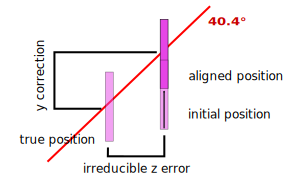
\includegraphics[width=\linewidth]{me13_motion.png}

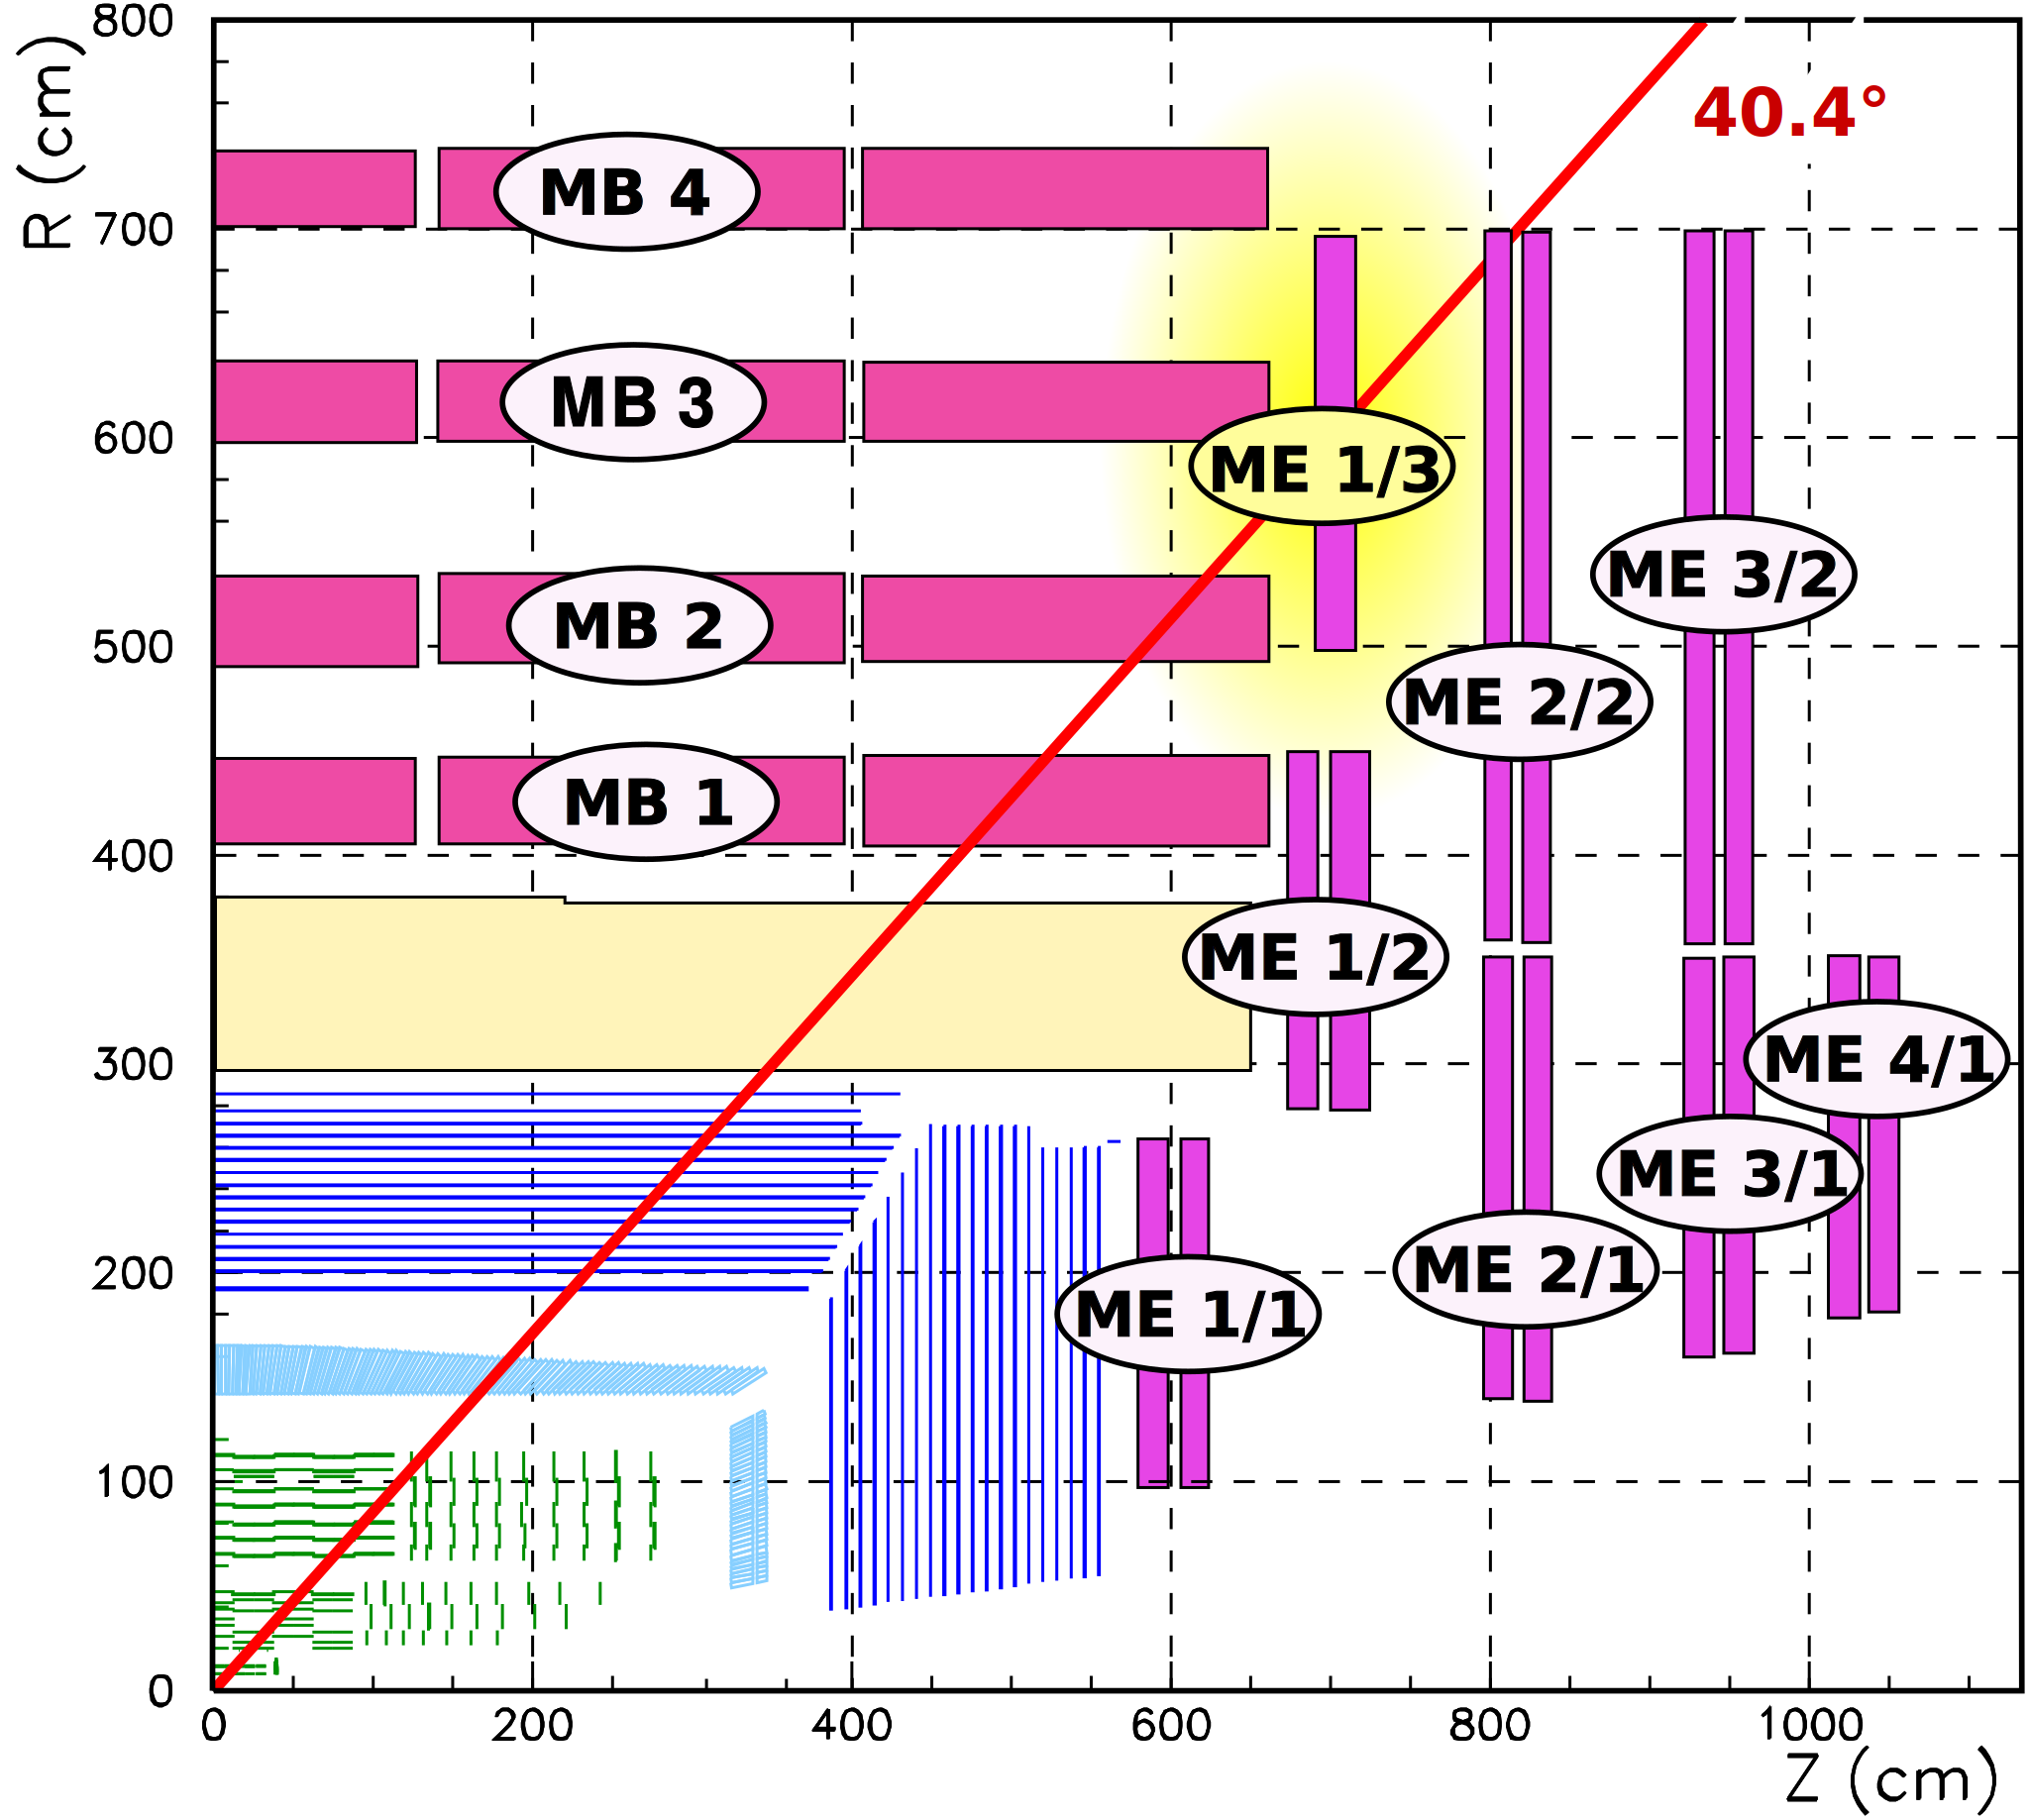
\includegraphics[width=\linewidth]{muon_system_highlight.png}

\column{0.5\linewidth}

\small
\begin{itemize}\setlength{\itemsep}{-0.02 cm}
\item Only I.P.\ muons in CSA
\item Chamber motion along line of sight cannot be determined
\item Fix $z$ and allow radial $y$ to float
\item Observed systematic shift in outer rings, also fixed $y$ in CSA
\item We now understand this shift
\item Ideally, resolve with cosmic rays
\end{itemize}

\includegraphics[height=\linewidth, angle=90]{corrected_me13y.pdf}

\end{columns}
\end{frame}

\begin{frame}
\frametitle{CSC overlaps procedure status}

\begin{itemize}\setlength{\itemsep}{0.4 cm}
\item Made MuAlOverlaps skims of CSA08 beam-halo MC
\item Solved some problems by looking at residuals with
test-misalignments
\begin{itemize}
\item e.g.\ two peaks when there should be one
\item large CSA statistics has helped
\end{itemize}
\item Still some problems with convergence
\begin{itemize}
\item standing waves along the CSC ring?
\item need a way to dampen them?
\item still speculative!
\end{itemize}
\item New ideas on a mini-version of the algorithm that uses (and
checks) hardware-alignment information
\item Working with hardware alignment group to make a comparison in
either April~1--3 or beginning of CRUZET-I
\end{itemize}

\end{frame}

\begin{frame}
\frametitle{Future plans}
\small

\begin{itemize}
\item Documentation

\vspace{-0.1 cm}
\begin{columns}
\column{0.08\linewidth}
\column{0.3\linewidth}
\begin{itemize}\setlength{\itemsep}{-0.05 cm}
\item CSA08 twiki $\surd$
\item CSA08 note
\end{itemize}
\column{0.7\linewidth}
\begin{itemize}\setlength{\itemsep}{-0.05 cm}
\item Longer MuonHIP note
\item Effect on physics for Muon POG note
\end{itemize}
\end{columns}
\item Produce more physics-relevant scenarios (tracker and muon)
\begin{itemize}
\item Re-run with samples in proportion (some CSA samples are a factor of 2 too big)
\item Does 100~pb$^{-1}$ of $Z\to\mu\mu$ help tracker curvature measurement?
\item What happens if material budget/magnetic field description is wrong?  Do I need to raise $p_T$ cut?
\item Validating FastSim residuals distributions, maybe 100~pb$^{-1}$
from FastSim (especially if $p_T$ cut is higher)
\item Include cosmic rays!  (2\_0\_9 tracker-enriched sample, \mbox{$B_{\mbox{on}}$/$B_{\mbox{off}}$)\hspace{-1 cm}}
\end{itemize}
\item Prepare for a {\it real} alignment with CRUZET-III and CRAFT
\item More alignment quality checks with data (e.g.\ absolute $\Rightarrow$ relative)
\item Keep working on the CSC overlaps procedure
\item Think about muon curvature constraint in tracker alignment
\end{itemize}

\label{numpages}
\end{frame}

\end{document}
